\subsection{Smart Watches}
In recent years, smart watches and other wearable technology has become increasingly popular\cite{noauthor_wearables_nodate}. They have gone from simple step trackers to small computers on your wrist: being able to send and receive messages, make calls, and almost every other feature that smartphones have. 

% \begin{wrapfigure}{l}{0.5\textwidth}
%     \centering
%     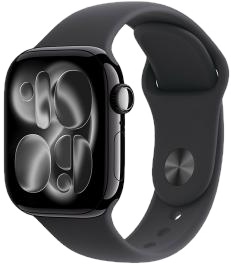
\includegraphics[width=0.5\linewidth]{report//images/Apple Watch.png}
%     \caption{Apple Watch Series 11}
%     \label{fig:smartwatch}
% \end{wrapfigure}

\wrapimage{r}
    {report//images/Apple Watch.png}
    {Apple Watch Series 11}
    {smartwatch}

Many modern smartwatches have evolved from early pedometers and fitness trackers, and therefor tend to incorporate inertial measurement units (IMUs) that could and are quite often already being used to detect falls\cite{noauthor_get_nodate, apple_watch_fall_detection, noauthor_samsung_nodate}. Most modern approaches to fall detection leverage these embedded sensors to detect motion patterns, often relying on machine learning or deep learning models. This section reviews several popular smartwatches, highlighting their strengths, limitations, and design considerations that we can take into consideration for the development our own solution. 



The next section is a comparison four of the most popular smartwatch brands\cite{statista_smartwatches} (as of May 2025)

\begin{longtable}{|p{3cm}|p{3cm}|p{3cm}|p{3cm}|p{3cm}|}

\hline
\textbf{Attribute} & \textbf{Apple Watch} (as seen in \ref{fig:smartwatch}) & \textbf{Huawei Watch} & \textbf{Samsung Galaxy Watch} & \textbf{Fitbit} \\
\hline
\endfirsthead

\hline
\textbf{Attribute} & \textbf{Apple Watch} & \textbf{Huawei Watch} & \textbf{Samsung Galaxy Watch} & \textbf{Fitbit} \\
\hline
\endhead
\hline
\multicolumn{5}{r}{\textit{(Continued)}} \\
\endfoot

\hline
\endlastfoot

Fall Detection & Yes (Series 4+) & Some models Yes & Some models Yes & Limited / No \\
\hline
Battery Life & 18-36 hours & 7-14 days & 2-4 days & 5-7 days \\
\hline
Heart Rate Monitoring & Yes & Yes & Yes & Yes \\
\hline
GPS & Yes & Yes & Yes & Yes \\
\hline
Price (Approx.) & \EUR{450} & \EUR{250} & \EUR{300} & \EUR{150} \\
\hline


\caption{Comparison of Popular Smartwatches} 
\label{tab:smartwatch_comparison} \\

\end{longtable}

% \subsubsection{Apple Watch}
% ** THIS NEEDS RE-WRITING **
% The Apple Watch\cite{apple_watch_fall_detection}, made by Apple, is a smart-watch filled with features to accompany you iPhone, AirPods or other Apple products. It has app's just like a normal smartphone, and many features built in for things like sleep- and workout tracking, music controls, voice assistants and many others.

% The Apple watch has for a couple of yeas now, had a feature in which it could detect emergencies and alert local emergency services and other emergency contacts, similarly to our idea. It boasts some other features that are only available in the Apple \textit{ecosystem} such as the relatives being able to track the victim in their "Find My" app, normally used to find other apple products and people. These extra features though cool, do come with a heavier price tag that other commercially available products. The Apple Watch is more intended to be setup for individual users, and not larger institutions such as retirement homes, or at home care since each user requires an Apple-id and an iPhone to connect it to.


% A reason you would choose an Apple Watch over other similar products could be because of its other features . But people that are at risk of falls, are usually in the elderly age-range, at might not have a need for all the bells and whistles of a whole smart watch.